\documentclass[aspectratio=169]{beamer}
\usepackage[T1]{fontenc}
\usepackage[utf8]{inputenc}
\usepackage{lmodern}
\usepackage{microtype}
\usepackage{xcolor}
\usepackage{tikz}
\usetikzlibrary{positioning, arrows.meta, calc}
\usepackage{fontawesome5}
\definecolor{wurgreen}{HTML}{34B233}
\definecolor{darkgreen}{HTML}{1F6B1E}
\definecolor{darknavy}{HTML}{1A1A2E}
\definecolor{midgray}{HTML}{6B7280}
\definecolor{lightgray}{HTML}{F3F4F6}
\definecolor{lightgreen}{HTML}{E8F7E8}
\definecolor{bodytext}{HTML}{1F2937}
\definecolor{warnred}{HTML}{FEE2E2}
\definecolor{warnborder}{HTML}{EF4444}
\definecolor{codebg}{HTML}{1E1E2E}
\definecolor{codegreen}{HTML}{9ECE6A}
\definecolor{codeblue}{HTML}{7AA2F7}
\definecolor{codeorange}{HTML}{FF9E64}
\definecolor{codegray}{HTML}{C0CAF5}
\usetheme{default}\usecolortheme{default}\usefonttheme{professionalfonts}
\setbeamertemplate{navigation symbols}{}
\setbeamertemplate{itemize items}{\textcolor{wurgreen}{\textbullet}}
\setbeamertemplate{itemize subitem}{\textcolor{midgray}{--}}
\setbeamercolor{frametitle}{fg=white, bg=darknavy}
\setbeamerfont{frametitle}{size=\large, series=\bfseries}
\setbeamertemplate{frametitle}{%
  \begin{beamercolorbox}[wd=\paperwidth, ht=1.1cm, dp=0.2cm, leftskip=0.6cm]{frametitle}
    \usebeamerfont{frametitle}\insertframetitle\end{beamercolorbox}}
\setbeamercolor{background canvas}{bg=white}
\setbeamercolor{normal text}{fg=bodytext}
\setbeamertemplate{footline}{%
  \begin{beamercolorbox}[wd=\paperwidth, ht=0.4cm, dp=0.15cm]{footline}
    \hspace{0.5cm}\textcolor{midgray}{\tiny Introduction to Python · Module 6: NumPy}%
    \hfill\textcolor{midgray}{\tiny \insertframenumber}\hspace{0.4cm}\end{beamercolorbox}}
\newcommand{\codebox}[1]{\begin{center}
  \begin{tikzpicture}\node[fill=codebg, rounded corners=4pt, inner sep=9pt, text width=0.85\textwidth, text=codegray]{\ttfamily\small #1};\end{tikzpicture}\end{center}}
\begin{document}
{\setbeamertemplate{footline}{}
\begin{frame}[plain]
  \begin{tikzpicture}[remember picture, overlay]
    \fill[darknavy] (current page.south west) rectangle (current page.north east);
    \fill[wurgreen] (current page.south west) rectangle ([xshift=0.45cm]current page.north west);
    \node[anchor=west, text=white, font=\huge\bfseries, text width=13cm] at ([xshift=1.1cm, yshift=1.4cm]current page.west){Introduction to Python};
    \node[anchor=west, text=wurgreen, font=\large, text width=12cm] at ([xshift=1.1cm, yshift=0.2cm]current page.west){Module 6 --- NumPy};
    \node[anchor=west, text=midgray, font=\small, text width=12cm] at ([xshift=1.1cm, yshift=-1.3cm]current page.west){Arrays and fast numerical computing};
  \end{tikzpicture}
\end{frame}}

\begin{frame}{What Is NumPy?}
\vspace{0.2cm}
{\small \textbf{NumPy} is the foundation of numerical computing in Python. Its core object is the
\textbf{array}: like a list, but built for \textbf{fast math} on lots of numbers at once.}
\medskip
\codebox{%
\textcolor{codeblue}{import} numpy \textcolor{codeblue}{as} np\\[6pt]
arr \textcolor{codegray}{=} np.\textcolor{codeblue}{array}([\textcolor{codeorange}{1}, \textcolor{codeorange}{2}, \textcolor{codeorange}{3}, \textcolor{codeorange}{4}])\\
\textcolor{codeblue}{print}(arr)\quad\ \ \ \ \ \ \textcolor{codegray}{\# [1 2 3 4]}\\
\textcolor{codeblue}{print}(arr.shape)\quad\textcolor{codegray}{\# (4,)  -- 4 elements}}
\medskip
{\small \texttt{import numpy as np} is the universal convention --- everyone writes \texttt{np}.
Nearly every data library (including pandas) is built on NumPy underneath.}
\end{frame}

\begin{frame}{Why Arrays Beat Lists for Math}
\vspace{0.2cm}
{\small The magic: operations apply to the \textbf{whole array at once} (``vectorization'') ---
no loop needed, and far faster.}
\medskip
\codebox{%
arr \textcolor{codegray}{=} np.\textcolor{codeblue}{array}([\textcolor{codeorange}{1}, \textcolor{codeorange}{2}, \textcolor{codeorange}{3}, \textcolor{codeorange}{4}])\\[6pt]
arr \textcolor{codegray}{*} \textcolor{codeorange}{2}\quad\ \ \ \textcolor{codegray}{\# [2 4 6 8]   -- every element doubled}\\
arr \textcolor{codegray}{+} \textcolor{codeorange}{10}\quad\ \textcolor{codegray}{\# [11 12 13 14]}\\
arr \textcolor{codegray}{**} \textcolor{codeorange}{2}\quad\ \textcolor{codegray}{\# [1 4 9 16]}}
\medskip
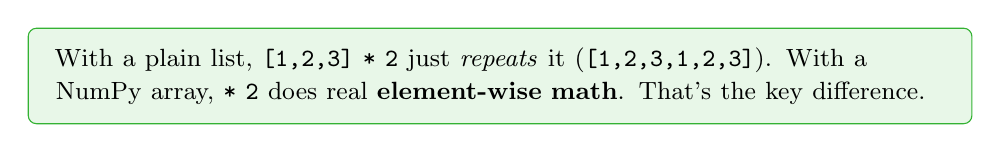
\begin{tikzpicture}
  \node[fill=lightgreen, draw=wurgreen, rounded corners=3pt, inner xsep=10pt, inner ysep=7pt, text width=\textwidth-24pt]{%
    {\small With a plain list, \texttt{[1,2,3] * 2} just \emph{repeats} it (\texttt{[1,2,3,1,2,3]}).
    With a NumPy array, \texttt{* 2} does real \textbf{element-wise math}. That's the key
    difference.}};
\end{tikzpicture}
\end{frame}

\begin{frame}{Useful Array Operations}
\vspace{0.2cm}
{\small NumPy has fast built-in summaries --- the bread and butter of data analysis.}
\medskip
\codebox{%
data \textcolor{codegray}{=} np.\textcolor{codeblue}{array}([\textcolor{codeorange}{4}, \textcolor{codeorange}{8}, \textcolor{codeorange}{15}, \textcolor{codeorange}{16}, \textcolor{codeorange}{23}])\\[6pt]
data.\textcolor{codeblue}{sum}()\quad\ \ \textcolor{codegray}{\# 66}\\
data.\textcolor{codeblue}{mean}()\quad\ \textcolor{codegray}{\# 13.2}\\
data.\textcolor{codeblue}{max}()\quad\ \ \textcolor{codegray}{\# 23}\\
data.\textcolor{codeblue}{std}()\quad\ \ \textcolor{codegray}{\# standard deviation}\\[6pt]
data[data \textcolor{codegray}{>} \textcolor{codeorange}{10}]\quad\textcolor{codegray}{\# [15 16 23]  -- filter by condition!}}
\medskip
{\small That last line --- \textbf{boolean filtering} --- is incredibly powerful: keep only the
elements that meet a condition. pandas uses the exact same idea on tables.}
\end{frame}

\begin{frame}{Module 6: Takeaways}
\vspace{0.3cm}
\begin{itemize}\setlength\itemsep{8pt}
  \item[\textcolor{wurgreen}{\faCheck}] \texttt{import numpy as np} --- the standard convention
  \item[\textcolor{wurgreen}{\faCheck}] A NumPy \textbf{array} is like a list, but built for fast numerical math
  \item[\textcolor{wurgreen}{\faCheck}] Operations are \textbf{vectorized}: \texttt{arr * 2} acts on every element
  \item[\textcolor{wurgreen}{\faCheck}] Built-in summaries: \texttt{.sum() .mean() .max() .std()}
  \item[\textcolor{wurgreen}{\faCheck}] \textbf{Boolean filtering} \texttt{arr[arr > 10]} keeps matching elements
\end{itemize}
\medskip
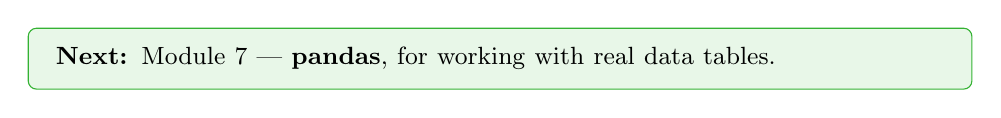
\begin{tikzpicture}
  \node[fill=lightgreen, draw=wurgreen, rounded corners=3pt, inner xsep=10pt, inner ysep=7pt, text width=\textwidth-24pt]{%
    {\small \textbf{Next:} Module 7 --- \textbf{pandas}, for working with real data tables.}};
\end{tikzpicture}
\end{frame}
\end{document}
